% =====================================================================
%  Web Mining Project Proposal
%  Skill Demand in Vietnam's IT and Business Analyst Job Postings
%
%  Compile with pdfLaTeX (Overleaf default) or run:
%      latexmk -pdf proposal.tex
%  Vietnamese characters are supported through the T5 font encoding.
%
%  >>> EDIT THE "TEAM INFORMATION" BLOCK BELOW TO FILL IN NAMES/IDs <<<
% =====================================================================
\documentclass[12pt,a4paper]{article}

% ---------- Encoding and fonts (Vietnamese support) ------------------
\usepackage[T5]{fontenc}        % T5 = Vietnamese font encoding
\usepackage[utf8]{inputenc}
\usepackage{lmodern}
\usepackage[english]{babel}

% ---------- Layout ---------------------------------------------------
\usepackage[a4paper,left=3cm,right=2cm,top=2.5cm,bottom=2.5cm]{geometry}
\usepackage{setspace}
\setstretch{1.2}
\usepackage{parskip}
\usepackage{titlesec}
\usepackage{fancyhdr}

% ---------- Tables, figures, math ------------------------------------
\usepackage{graphicx}
\usepackage{booktabs}
\usepackage{tabularx}
\usepackage{array}
\usepackage{longtable}
\usepackage{multirow}
\usepackage{enumitem}
\usepackage{amsmath,amssymb}
\usepackage{xcolor}
\usepackage{tikz}
\usetikzlibrary{arrows.meta,positioning,shapes.geometric}
\usepackage{caption}
\usepackage{float}              % [H] keeps tables next to their section
\usepackage[hidelinks,pdfpagelabels]{hyperref}

\newcolumntype{L}{>{\raggedright\arraybackslash}X}
\newcolumntype{P}[1]{>{\raggedright\arraybackslash}p{#1}}
\setlist{nosep,leftmargin=1.5em}
\captionsetup{font=small,labelfont=bf}

\titleformat{\section}{\large\bfseries}{\thesection.}{0.6em}{}
\titleformat{\subsection}{\normalsize\bfseries}{\thesubsection.}{0.6em}{}

% =====================================================================
%  TEAM INFORMATION  ---  replace the placeholder text below
% =====================================================================
\newcommand{\University}{ĐẠI HỌC BÁCH KHOA HÀ NỘI}
\newcommand{\UniversityEN}{HANOI UNIVERSITY OF SCIENCE AND TECHNOLOGY}
\newcommand{\SchoolEN}{School of Information and Communication Technology}
\newcommand{\CourseName}{Web Mining (Khai phá Web)}
\newcommand{\CourseCode}{IT4868}
\newcommand{\Semester}{Semester 2026.1}
\newcommand{\GroupNo}{Group 1}
\newcommand{\Place}{Hà Nội}
\newcommand{\SubmitDate}{\today}

% Supervisor (e.g. "PGS.TS. Nguyễn Văn A")
\newcommand{\SupervisorName}{TS. Dương Quang Huy}

% Students: full Vietnamese name and student ID (MSSV)
\newcommand{\StudentOneName}{Nguyễn Trần Minh Trí}
\newcommand{\StudentOneID}{202400116}
\newcommand{\StudentTwoName}{Tô Duy An}
\newcommand{\StudentTwoID}{202416653}
\newcommand{\StudentThreeName}{Kiều Việt Sơn}
\newcommand{\StudentThreeID}{202416750}
\newcommand{\StudentFourName}{Nguyễn Ngọc Tuấn Anh}
\newcommand{\StudentFourID}{202416659}

\newcommand{\ProjectTitle}{Skill Demand in Vietnam's IT and Business Analyst
Job Postings: A Text Mining Study, 2020--2025}

% ---------- Header / footer ------------------------------------------
\pagestyle{fancy}
\fancyhf{}
\fancyhead[L]{\small \CourseCode\ -- \CourseName}
\fancyhead[R]{\small Project Proposal}
\fancyfoot[C]{\thepage}
\renewcommand{\headrulewidth}{0.4pt}
\setlength{\headheight}{15pt}

\hypersetup{pdftitle={Project Proposal: Skill Demand in Vietnam IT and BA Job Postings}}

% =====================================================================
\begin{document}

% ============================ COVER PAGE =============================
\pagenumbering{Alph}  % unique page anchors for the cover page
\begin{titlepage}
  \thispagestyle{empty}
  \setstretch{1.0}
  \setlength{\parskip}{0pt}
  \centering
  {\large\bfseries \University\par}
  {\normalsize \UniversityEN\par}
  \vspace{0.25cm}
  {\normalsize\bfseries \SchoolEN\par}
  \vspace{0.15cm}
  \rule{0.6\textwidth}{0.8pt}\par
  \vspace{0.6cm}

  % Place the logo file "hust_logo.png" next to this .tex file to show it
  \IfFileExists{hust_logo.png}{%
    
\includegraphics[height=2.8cm]{hust_logo.png}\par}{%
    \fbox{\parbox[c][2.6cm][c]{3.0cm}{\centering\small\color{gray}HUST logo\\(hust\_logo.png)}}\par}
  \vspace{0.6cm}

  {\Large\bfseries PROJECT PROPOSAL\par}
  \vspace{0.2cm}
  {\large Course: \CourseName\ -- \CourseCode\par}
  \vspace{0.1cm}
  {\normalsize \Semester\par}
  \vspace{0.6cm}

  {\Large\bfseries \setstretch{1.15}\ProjectTitle\par}
  \vspace{0.8cm}

  \begin{flushleft}
  \begin{tabular}{@{}ll@{}}
    \textbf{Supervisor:} & \SupervisorName \\[4pt]
    \textbf{Team:}       & \GroupNo \\
  \end{tabular}
  \end{flushleft}

  \vspace{0.2cm}
  \renewcommand{\arraystretch}{1.45}
  \begin{tabularx}{\textwidth}{|c|L|>{\centering\arraybackslash}p{4.2cm}|}
    \hline
    \textbf{No.} & \textbf{Full name (Họ và tên)} & \textbf{Student ID (MSSV)} \\
    \hline
    1 & \StudentOneName   & \StudentOneID   \\ \hline
    2 & \StudentTwoName   & \StudentTwoID   \\ \hline
    3 & \StudentThreeName & \StudentThreeID \\ \hline
    4 & \StudentFourName  & \StudentFourID  \\ \hline
  \end{tabularx}
  \renewcommand{\arraystretch}{1.0}

  \vfill
  {\large \Place, \SubmitDate\par}
\end{titlepage}

% ============================ CONTENTS ===============================
\pagenumbering{roman}
\tableofcontents
\clearpage
\pagenumbering{arabic}

% ============================ ABSTRACT ===============================
\section*{Abstract}
\addcontentsline{toc}{section}{Abstract}

Employers describe job requirements in free text, using inconsistent
spellings, abbreviations, and a mix of Vietnamese and English for the same
skill. This makes it difficult to compare skill demand across roles or to
monitor how requirements change over time. This project proposes a
reproducible Web Mining pipeline that identifies Information Technology (IT)
and Business Analyst (BA) postings in a research-permitted Vietnamese
job-advertisement corpus, extracts skill mentions, maps aliases to canonical
skill names, and analyzes skill prevalence and co-occurrence by role,
location, and period (target window 2020--2025, subject to verified data
coverage).

Skills will be extracted with an interpretable bilingual dictionary baseline
and compared with a PhoBERT-based sequence-labeling model; a manually
annotated gold sample will be used to measure precision, recall, and F1. The
normalized skills will then be summarized as posting-level prevalence and as
separate IT and BA skill co-occurrence networks. Deliverables include a
cleaned analysis dataset, a versioned skill vocabulary, extraction and
evaluation code, and visualizations. Findings will describe the sampled
postings and will not be presented as a complete measure of the Vietnamese
labor market.

\textbf{Keywords:} web mining, text mining, information extraction, skill
extraction, job postings, co-occurrence network, PhoBERT, Vietnam.

% ============================ 1. INTRODUCTION ========================
\section{Introduction}

\subsection{Background and motivation}
Online job advertisements are a rich source of evidence about how employers
express role requirements. A single paragraph may mention programming
languages, frameworks, cloud platforms, analysis methods, certifications, and
interpersonal capabilities. In Vietnam, postings for technology roles are
frequently written in Vietnamese, in English, or in a mixture of both, and
the same skill may appear under several surface forms (for example
\emph{JS}, \emph{Javascript}, and \emph{JavaScript}; and \emph{business analysis}).

A simple word count therefore overstates some skills, misses aliases, and
makes comparisons between job families unreliable. Students, training
programs, and job seekers benefit from a transparent and evaluated
description of which skills are requested together and how this differs
between IT and BA roles.

\subsection{Problem statement}
Job requirements are mostly unstructured and vary in wording and language
across employers and platforms. Without a consistent method for identifying
and normalizing skills, comparisons of demand by role, location, or time can
be misleading. This project assesses whether a practical extraction and
normalization pipeline can produce sufficiently accurate skill data for
descriptive analysis of Vietnamese IT and BA postings, and uses that data to
show how skill combinations differ across job families.

% ============================ 2. AIM / OBJECTIVES / RQ ================
\section{Aim, Objectives, and Research Questions}

\subsection{Aim}
To develop and evaluate a reproducible pipeline for extracting, normalizing,
and analyzing skills in Vietnamese IT and BA job postings.

\subsection{Objectives}
\begin{enumerate}
  \item Select a research-permitted Vietnamese job-posting dataset and define
        a focused sampling frame with verified date coverage.
  \item Identify IT and BA postings using transparent title rules, validated
        on a manually labeled sample, with an optional machine-learning
        classifier.
  \item Extract skill mentions from posting text using a bilingual skill
        vocabulary and a neural sequence-labeling model.
  \item Normalize aliases and spelling variants to canonical skill labels
        while keeping the original mentions for auditability.
  \item Evaluate extraction quality against a manually annotated gold sample
        using precision, recall, and F1.
  \item Compare skill prevalence and co-occurrence across job families,
        broad locations, and time periods where the data supports it.
\end{enumerate}

\subsection{Research questions}
\begin{description}[leftmargin=3.2em,style=nextline]
  \item[RQ1.] Which skills are most frequently requested in Vietnamese IT and
        BA postings during the study period?
  \item[RQ2.] Which skills tend to appear together, and how do these
        combinations differ between IT and BA roles?
  \item[RQ3.] Where location and date coverage are adequate, how does
        observed skill demand vary across broad locations and years?
  \item[RQ4.] How accurately do the dictionary baseline and the neural model
        identify skill mentions in a manually reviewed sample?
\end{description}

These are descriptive questions; the project makes no causal claims and does
not forecast future employment outcomes.

% ============================ 3. SCOPE ===============================
\section{Scope and Delimitations}

\begin{itemize}
  \item \textbf{Geography:} jobs advertised for work in Vietnam; national
        results first, then broad locations (Hà Nội, TP.~Hồ Chí Minh,
        Đà Nẵng, other/unspecified) when sample sizes allow.
  \item \textbf{Time:} target January 2020 -- December 2025. The final window
        will follow the chosen source's verified coverage; if historical
        years are missing, the study is shortened or reframed as a snapshot.
  \item \textbf{Job families:} IT (software, data/AI, QA/testing,
        infrastructure/cloud/security) and BA (business analyst, IT/business
        systems analyst, process analyst). Boundary roles such as Data
        Analyst, Product Owner, and Project Manager will be explicitly
        included or excluded in a documented role-mapping table.
  \item \textbf{Language:} Vietnamese, English, and mixed postings; the
        language of each posting is recorded and analyzed.
  \item \textbf{Outcome:} percentage of postings requesting each skill and
        co-occurring skill combinations. Salary and experience are optional
        and used only if consistently available.
  \item \textbf{Out of scope:} inferring a person's qualifications,
        predicting hiring outcomes, ranking candidates, or treating
        advertisement counts as total employment demand.
\end{itemize}

% ============================ 4. DATA PLAN ===========================
\section{Data Plan}
This is just the draft we made, after trying this approch, we may alter it.
\subsection{Candidate data sources}
Table~\ref{tab:sources} lists the candidate sources. A dataset is not
automatically reusable just because it is publicly downloadable; license,
provenance, and coverage will be verified before selection. Existing
datasets are preferred for historical coverage; manual collection from job
boards (Section~\ref{sec:manual}) is the supplementary source and the
fallback for a recent snapshot.

\begin{table}[H]
\centering\small
\caption{Candidate data sources}
\label{tab:sources}
\begin{tabularx}{\textwidth}{@{}P{3.3cm}LL@{}}
\toprule
\textbf{Source} & \textbf{Potential use} & \textbf{Checks / limitations} \\
\midrule
VietJobs dataset~\cite{vietjobs} & Primary candidate; reported 48{,}092
  Vietnamese job ads with title, category, salary, and skill fields &
  Confirm release location, license, date range, duplicate policy, and
  availability of full descriptions \\
\addlinespace
VietJobs-37K / VieJobBERT~\cite{viejobbert} & Role-classification
  benchmark and supplementary Vietnamese text (37{,}274 postings, 60
  occupation labels) & Not designed as a longitudinal skills dataset; check
  Zenodo license and fields; silver labels are keyword-derived \\
\addlinespace
Techmap / JobDataFeeds~\cite{techmap} & Historical postings since January
  2020 with title, description, location, skills & Paid product; confirm
  academic license, redistribution limits, and exact coverage \\
\addlinespace
University / instructor archive & Preferred if available & Obtain written
  permission, collection dates, and field definitions \\
\addlinespace
TopCV (manual collection) & Primary board for manual collection; large
  Vietnamese board with IT and BA categories, full job descriptions,
  location, and posting/expiry dates & Verify Terms of Service and
  robots.txt; active postings only (no history); ranking and platform bias
  \\
\addlinespace
ITviec / TopDev (manual collection) & IT-focused boards; skill tags and
  full descriptions, many bilingual postings & Verify terms; IT-heavy, few
  BA postings; some content may need login (not used if so) \\
\addlinespace
VietnamWorks / CareerViet (manual collection) & Optional extra boards to
  balance BA postings and locations & Verify terms; check that fields
  match other boards before merging \\
\addlinespace
LinkedIn (optional, manual only) & Small validation sample of
  English-language postings & User agreement restricts automated
  collection and most content is login-gated; no scripts, no login bypass;
  dropped if terms do not allow research use \\
\bottomrule
\end{tabularx}
\end{table}

\textbf{Selection sequence.} (1) Ask the supervisor or library for an
existing permitted archive; (2) inspect the VietJobs and VietJobs-37K
releases and terms; (3) request a sample and academic terms from the
commercial provider if budget allows; (4) in parallel, run the manual
collection of Section~\ref{sec:manual} for a recent snapshot from boards
whose terms allow it; (5) otherwise narrow the period to a source that can
be accessed lawfully. Sources will not be merged until their fields, dates,
and collection methods are comparable.

\subsection{Manual collection from job boards}\label{sec:manual}
Public datasets may not cover 2020--2025 with full descriptions and dates.
To ensure that the project always has usable text, the team will build a
small, documented snapshot corpus by manual or semi-manual collection from
Vietnamese job boards. Because boards show mainly active postings, this
corpus supports prevalence, co-occurrence, and location analyses for the
collection period only. Year-by-year trends use it only where the board
shows a reliable posting date, and otherwise rely on the historical dataset.

\textbf{Source priority.} TopCV and ITviec/TopDev first (large Vietnamese
boards with full descriptions); VietnamWorks/CareerViet to add BA
postings; LinkedIn only as an optional, manually collected validation
sample.

\textbf{Compliance protocol.}
\begin{enumerate}
  \item Before collecting from a board, read its Terms of Service and
        \texttt{robots.txt}, and record the date, the URL of the terms, and
        the decision (allowed / not allowed / unclear) in the source
        register. Unclear is treated as not allowed unless the supervisor
        or the site gives written permission.
  \item Use only public pages. No login, no CAPTCHA or rate-limit
        circumvention, no private or applicant-side data.
  \item Collection is done by a team member browsing the listing pages and
        saving each page or copying fields into a structured sheet. Where
        the terms permit scripts, a single-threaded script with a
        descriptive user agent and delays of several seconds between
        requests may be used. Collection stops if a site blocks or warns
        the client.
  \item Raw pages stay private, are not redistributed, and are deleted or
        archived according to the course and supervisor rules; only
        aggregated results are published.
\end{enumerate}

\textbf{Sampling frame.} Searches use a fixed query list in Vietnamese
and English (e.g.\ \emph{Business Analyst}, \emph{phân tích nghiệp vụ},
\emph{Software Engineer}, \emph{Data Engineer}, \emph{QA/Tester},
\emph{DevOps}, \emph{Cloud/Security}) with location filters for Hà Nội,
TP.~Hồ Chí Minh, Đà Nẵng, and other. Collection is quota-based (a target
number of postings per role family $\times$ city $\times$ board, with BA
oversampled relative to its natural share) so that groups are large enough
to compare. Query terms, filters, collection dates, and counts are logged
for every run so that the sample can be described and repeated.

\textbf{Collected fields.}

\begin{table}[H]
\centering\small
\caption{Fields captured during manual collection}
\label{tab:crawlfields}
\begin{tabularx}{\textwidth}{@{}P{3.6cm}P{4.4cm}L@{}}
\toprule
\textbf{Field} & \textbf{Purpose} & \textbf{Handling} \\
\midrule
Source board, URL, collection date & Provenance and repost checks & URL
  stored as a hash in the shared dataset \\
Job title & IT/BA family & Kept verbatim \\
Description sections & Skill extraction & Requirements, responsibilities,
  and benefits saved separately where the page allows \\
Skill tags (if shown) & Weak labels and vocabulary seeding & Kept apart from
  the gold annotations \\
Posting date / expiry & Period assignment & Missing values kept as missing \\
Location & Regional comparison & Mapped to broad regions \\
Company name & Cross-board deduplication & Used only for matching, then
  dropped from the analysis dataset \\
Salary (optional) & Descriptive only & Only if explicit \\
Source board & Platform-effect checks & Stored per posting \\
\bottomrule
\end{tabularx}
\end{table}

\textbf{Quality and bias controls.}
\begin{itemize}
  \item Remove exact duplicates and flag cross-board reposts (title,
        company, location, and text similarity).
  \item Report the number of postings per board, role, city, and month;
        analyze results per board to show platform effects.
  \item Acknowledge that listing order, active-only visibility, and each
        board's employer mix bias the sample; do not describe the corpus
        as the whole market.
  \item Treat the manual corpus as the evaluation and annotation pool,
        with the historical dataset used for scale where it is available.
\end{itemize}

\subsection{Project fields}

\begin{table}[H]
\centering\small
\caption{Fields used in the analysis dataset}
\label{tab:fields}
\begin{tabularx}{\textwidth}{@{}P{3.4cm}P{4.2cm}L@{}}
\toprule
\textbf{Field} & \textbf{Purpose} & \textbf{Handling} \\
\midrule
Posting ID & Deduplication and joins & Replaced by a generated project ID \\
Job title & Assign IT/BA family & Normalized separately from description \\
Description / requirements & Skill extraction & Processed locally; contact
  details removed \\
Posting date & Trend summaries & ISO date, derived year/quarter; missingness kept \\
Location & Regional comparison & Mapped to broad regions; unknown kept separate \\
Language & Coverage analysis & Vietnamese / English / mixed label \\
Salary (optional) & Descriptive only & Used only if period and currency are explicit \\
\bottomrule
\end{tabularx}
\end{table}

\subsection{Data preparation}
\begin{enumerate}
  \item Build a raw-data inventory and profile missingness, text length, and
        encoding issues by year and source.
  \item Standardize core fields; remove exact duplicates and flag likely
        reposts using title, company, location, date proximity, and text
        similarity.
  \item Normalize dates and locations; detect language (Vietnamese, English,
        mixed) and audit a sample manually.
  \item Mask e-mail addresses, phone numbers, and personal names that are not
        needed for analysis.
  \item Record row counts after every filter in a cleaning audit so the
        analysis can be reproduced.
\end{enumerate}

% ============================ 5. METHODOLOGY =========================
\section{Methodology}

\subsection{Pipeline overview}
Figure~\ref{fig:pipeline} summarizes the proposed pipeline. Occupation
classification (what kind of job a posting describes) and skill-span
extraction (which skills a posting mentions) are kept as separate tasks so
that each can be evaluated independently.

\begin{figure}[H]
\centering
\setstretch{1.0}\hyphenpenalty=10000
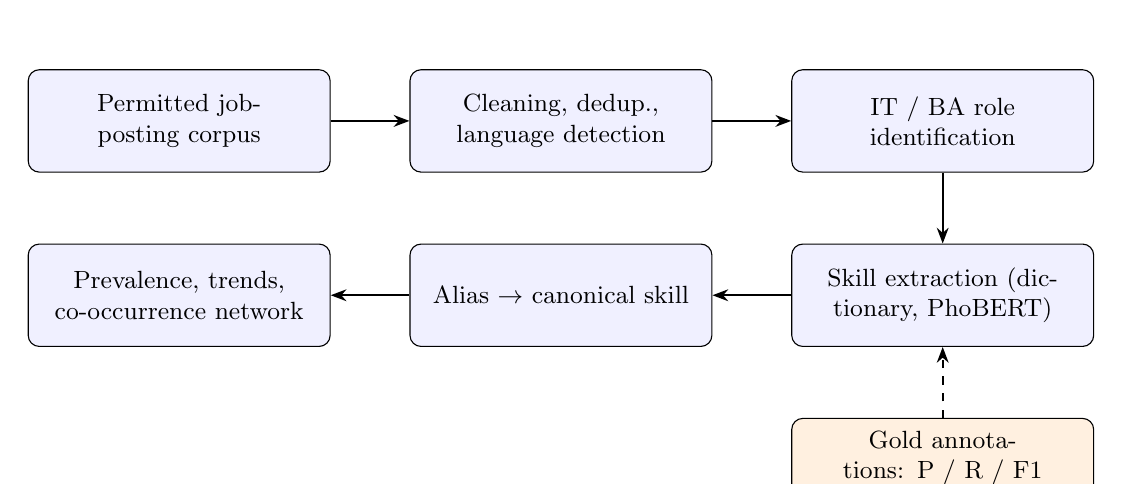
\begin{tikzpicture}[
  node distance=0.9cm and 1.0cm,
  box/.style={draw,rounded corners,fill=blue!6,align=center,
              minimum height=1.3cm,text width=3.6cm,font=\small},
  eval/.style={draw,rounded corners,fill=orange!12,align=center,
              minimum height=1.0cm,text width=3.6cm,font=\small},
  arr/.style={-{Stealth[length=2mm]},thick}]
  \node[box] (data) {Permitted job-posting corpus};
  \node[box,right=of data] (clean) {Cleaning, dedup., language detection};
  \node[box,right=of clean] (role) {IT / BA role identification};
  \node[box,below=of role] (skill) {Skill extraction (dictionary, PhoBERT)};
  \node[box,left=of skill] (norm) {Alias $\rightarrow$ canonical skill};
  \node[box,left=of norm] (mine) {Prevalence, trends, co-occurrence network};
  \node[eval,below=of skill] (gold) {Gold annotations: P / R / F1};
  \draw[arr] (data) -- (clean);
  \draw[arr] (clean) -- (role);
  \draw[arr] (role) -- (skill);
  \draw[arr] (skill) -- (norm);
  \draw[arr] (norm) -- (mine);
  \draw[arr,dashed] (gold) -- (skill);
\end{tikzpicture}
\caption{Proposed skill-mining pipeline}
\label{fig:pipeline}
\end{figure}

\subsection{IT and BA job-family identification}
A title taxonomy with aliases will be drafted, including rules for ambiguous
roles (e.g.\ \emph{Data Analyst} is not automatically a BA role). A stratified
sample of titles will be labeled as IT, BA, both, other, or uncertain, with a
second reviewer labeling a subset to measure agreement. The baseline is a set
of transparent keyword rules; an optional classifier uses word/character
TF--IDF with logistic regression or a linear SVM, or a fine-tuned
PhoBERT~\cite{phobert} model (we may use another model or customize another baseline later) if enough labeled data is available. Results are
reported as macro-F1, per-class precision/recall/F1, and a confusion matrix.

\subsection{Skill vocabulary and annotation}
A versioned bilingual vocabulary will record, for each entry, a canonical
label, aliases, language, category (programming languages, frameworks,
cloud/\allowbreak DevOps, data/\allowbreak AI, testing/\allowbreak security,
databases, BA methods, requirements/\allowbreak process, tools,
communication/\allowbreak domain skills), source, and
ambiguity notes. ESCO~\cite{esco} and O*NET~\cite{onet} are used as
supplementary references only, because neither is a Vietnam-specific
taxonomy and ESCO has no Vietnamese language pack. A written annotation guide
will define span boundaries, lists, acronyms, negation, and the distinction
between required and preferred skills. A stratified sample (by role, period,
and language) will be annotated, with a double-labeled subset used to report
inter-annotator agreement.

\subsection{Skill extraction models}

\begin{table}[H]
\centering\small
\caption{Extraction approaches compared}
\label{tab:models}
\begin{tabularx}{\textwidth}{@{}P{3.6cm}P{2.6cm}L@{}}
\toprule
\textbf{Approach} & \textbf{Role} & \textbf{Notes} \\
\midrule
Dictionary / phrase matching & Required baseline & Boundary-aware,
  interpretable, easy to audit; misses unseen forms \\
PhoBERT token classification (BIO) & Main neural model & Context-sensitive
  Vietnamese representation~\cite{phobert}; predicts exact spans \\
XLM-R token classification & Optional & For substantially mixed
  Vietnamese--English text~\cite{xlmr} \\
CRF / BiLSTM-CRF & Optional & Traditional sequence-labeling comparison \\
Embedding-based linking & Optional & Suggests canonical labels for unseen
  phrases; always manually validated \\
\bottomrule
\end{tabularx}
\end{table}

Data are split by posting, keeping likely duplicates in the same split; if
the sample allows, the latest year is reserved as a temporal test set. The
untouched test set is used only for final reporting.

\subsection{Evaluation of extraction}
Let $TP$, $FP$, and $FN$ denote true positives, false positives, and false
negatives with respect to the adjudicated gold spans. We report
\begin{equation}
  P = \frac{TP}{TP+FP}, \qquad
  R = \frac{TP}{TP+FN}, \qquad
  F_1 = \frac{2PR}{P+R},
\end{equation}
for exact-span and relaxed-overlap matching, together with canonical-skill
micro and macro F1, per-category and per-language results, and support
counts.

\subsection{Prevalence and co-occurrence analysis}
Let $D_g$ be the eligible postings in group $g$ (role, location, or period)
and $S(d)$ the set of canonical skills in posting $d$. The main demand
measure is posting prevalence:
\begin{equation}
  \text{prev}_g(s) = \frac{\left|\{\, d \in D_g : s \in S(d) \,\}\right|}{|D_g|}.
\end{equation}
For skills $a$ and $b$ with posting sets $D_a$ and $D_b$ among $N$ postings,
co-occurrence strength is measured with
\begin{equation}
  J(a,b) = \frac{|D_a \cap D_b|}{|D_a \cup D_b|}, \qquad
  \text{lift}(a,b) = \frac{N\,|D_a \cap D_b|}{|D_a|\,|D_b|}.
\end{equation}
Separate weighted, undirected networks will be built for IT and BA, with
nodes as canonical skills and edges above a documented minimum support.
Community detection and centrality are used as exploratory summaries, and
clusters are interpreted through their member skills. Time series are
aggregated by year or quarter and always shown with their denominators.

\subsection{Baselines and robustness checks}
\begin{itemize}
  \item Dictionary-only extraction versus the final model.
  \item Exact matching without alias normalization versus normalized output.
  \item Alternative duplicate filters, minimum-text rules, and edge-support
        thresholds.
  \item Results by language subset and by source composition per period.
\end{itemize}

% ============================ 6. EVALUATION CRITERIA =================
\section{Success Criteria}
The project will be considered successful if it:
\begin{enumerate}
  \item produces a traceable, documented mapping from surface forms to
        canonical skills;
  \item reports extraction precision, recall, and F1 on a manually reviewed
        sample;
  \item provides interpretable comparisons of skill prevalence and
        co-occurrence for IT and BA postings;
  \item documents sampling, data limitations, and processing decisions well
        enough for another student to reproduce the analysis.
\end{enumerate}
No minimum accuracy threshold is assumed in advance; weak results will be
reported and the analysis narrowed to reliably extracted skill groups.

% ============================ 7. ETHICS ==============================
\section{Ethics and Responsible Interpretation}
\begin{itemize}
  \item Follow dataset licenses and source terms; document the basis for
        access and use.
  \item Publish aggregated results only; do not redistribute raw posting text
        unless explicitly permitted.
  \item Remove personal contact details; collect no data about applicants or
        employees.
  \item Describe findings as patterns in the sampled postings, and report
        coverage, language, platform, and deduplication biases.
  \item Do not interpret an increase in mentions as proof of a causal change
        in employer needs.
\end{itemize}

% ============================ 8. TOOLS ===============================
\section{Tools and Implementation}
Python with \texttt{pandas} (data preparation), regular expressions or a
phrase matcher (dictionary baseline), Hugging Face \texttt{transformers}
(PhoBERT/XLM-R), \texttt{scikit-learn} (classifiers and metrics),
\texttt{networkx} (co-occurrence graphs), and \texttt{matplotlib}/
\texttt{seaborn} (visualization). The skill vocabulary is stored as a
versioned CSV/JSON file; configuration, random seeds, and parameters are kept
under version control (Git) alongside the code.

% ============================ 9. WORK PLAN ===========================
\section{Work Plan}

\begin{table}[H]
\centering\small
\caption{Nine-week timeline}
\label{tab:timeline}
\begin{tabularx}{\textwidth}{@{}c L P{4.2cm}@{}}
\toprule
\textbf{Week} & \textbf{Activities} & \textbf{Milestone} \\
\midrule
1 & Define scope, role families, time window; search candidate sources &
    Approved scope memo \\
2 & License and provenance checks; inspect samples; select primary source &
    Source decision record \\
3 & Data profiling, cleaning, deduplication, language detection &
    Clean dataset v1 and audit \\
4 & Title taxonomy and labeling; pilot-read postings for skills &
    Role guide, pilot notes \\
5 & Role rules/classifier; bilingual vocabulary; annotation of gold sample &
    Vocabulary v1, gold set \\
6 & Dictionary baseline; BIO data preparation; PhoBERT fine-tuning &
    Model predictions \\
7 & Extraction evaluation and error analysis; prevalence, trend, location,
    and network analyses & Evaluation table, figures \\
8 & Robustness checks; draft methods, results, and limitations &
    Findings memo, report draft \\
9 & Report integration, reproducibility review, presentation &
    Final report and slides \\
\bottomrule
\end{tabularx}
\end{table}

If time is short, the optional models (XLM-R, CRF) and salary analysis are
dropped before any reduction of the manual evaluation.

% ============================ 10. TEAM ===============================
\section{Division of Work}

\begin{table}[H]
\centering\small
\caption{Team roles and responsibilities}
\label{tab:team}
\begin{tabularx}{\textwidth}{@{}P{3.6cm} P{3.4cm} L@{}}
\toprule
\textbf{Member} & \textbf{Main responsibility} & \textbf{Outputs} \\
\midrule
\StudentOneName\newline(\StudentOneID) & Data and provenance & Source and
  license register, clean dataset, data-quality report, cleaning code \\
\addlinespace
\StudentTwoName\newline(\StudentTwoID) & IT/BA job-family classification &
  Role guide, labeled titles, rule baseline and classifier with metrics \\
\addlinespace
\StudentThreeName\newline(\StudentThreeID) & Skills and NLP & Bilingual
  vocabulary, gold annotations, dictionary and PhoBERT extraction,
  evaluation \\
\addlinespace
\StudentFourName\newline(\StudentFourID) & Mining and communication &
  Prevalence, trend, and network analyses; robustness checks; report and
  presentation integration \\
\bottomrule
\end{tabularx}
\end{table}

All members take part in the scope freeze, double annotation, results review,
and final presentation.

% ============================ 11. RISKS ==============================
\section{Risks and Mitigation}

\begin{table}[H]
\centering\small
\caption{Main risks}
\label{tab:risks}
\begin{tabularx}{\textwidth}{@{}P{4.0cm} P{3.4cm} L@{}}
\toprule
\textbf{Risk} & \textbf{Effect} & \textbf{Mitigation} \\
\midrule
Unclear license or provenance & Dataset unusable & Verify before analysis;
  switch to a permitted source \\
Missing years in the source & No valid trend analysis & Shorten the window
  or reframe as a snapshot \\
Short, missing, or duplicated text & Biased prevalence & Profile coverage,
  deduplicate, minimum-text rules, report exclusions \\
Ambiguous aliases, mixed language & Lower precision/recall & Boundary-aware
  matching, context rules, per-language evaluation \\
Inconsistent role labels & Mixed comparisons & Few families; validate rules
  on a labeled sample \\
Too few records per group & Unstable estimates & Merge groups, raise
  minimum support, or omit the comparison \\
Site terms forbid collection or the site blocks requests & Source unusable
  & Check terms first; stop on blocks; switch board or dataset \\
Snapshot-only boards & No historical trend & Report as a snapshot; use the
  historical dataset for years where it is verified \\
\bottomrule
\end{tabularx}
\end{table}

% ============================ 12. DELIVERABLES =======================
\section{Expected Deliverables}
\begin{enumerate}
  \item A data statement covering source, license, coverage, sampling, and
        limitations.
  \item A versioned bilingual skill vocabulary with aliases and ambiguity
        notes.
  \item A reproducible cleaning, role-identification, extraction, and
        normalization pipeline.
  \item A manually annotated gold sample with reported precision, recall,
        and F1.
  \item Tables and figures of skill prevalence by role, location, and period.
  \item IT and BA skill co-occurrence networks with interpretation.
  \item A final report, presentation, and README with reproduction steps.
\end{enumerate}

% ============================ 13. CONCLUSION =========================
\section{Conclusion}
This project turns unstructured Vietnamese job-advertisement text into an
auditable dataset of normalized skills, measures how reliably those skills
can be extracted, and applies Web Mining methods to describe skill demand and
skill combinations in IT and BA roles. Its focused scope, manual quality
check, and explicit account of data provenance make it feasible within one
semester while still producing measurable results.

% ============================ REFERENCES =============================
\begin{thebibliography}{9}
\addcontentsline{toc}{section}{References}

\bibitem{vietjobs}
\emph{VietJobs: A Vietnamese Job Advertisement Dataset}.
arXiv preprint arXiv:2603.05262.
\url{https://arxiv.org/abs/2603.05262}

\bibitem{viejobbert}
KALD Labs. \emph{VieJobBERT: VietJobs-37K dataset and benchmark code}.
\url{https://github.com/kaldlabs/VieJobBERT}

\bibitem{techmap}
Techmap. \emph{Vietnam job posting data}.
\url{https://jobdatafeeds.com/data/countries/vn}

\bibitem{phobert}
D.~Q. Nguyen and A.~T. Nguyen.
PhoBERT: Pre-trained language models for Vietnamese.
In \emph{Findings of the Association for Computational Linguistics: EMNLP
2020}, pp.~1037--1042, 2020.

\bibitem{xlmr}
A.~Conneau, K.~Khandelwal, N.~Goyal, et al.
Unsupervised cross-lingual representation learning at scale.
In \emph{Proceedings of the 58th Annual Meeting of the Association for
Computational Linguistics (ACL)}, pp.~8440--8451, 2020.

\bibitem{esco}
European Commission. \emph{ESCO: European Skills, Competences,
Qualifications and Occupations}.
\url{https://esco.ec.europa.eu/en/use-esco}

\bibitem{onet}
National Center for O*NET Development. \emph{O*NET license agreements}.
\url{https://www.onetcenter.org/license_agreements.html}

\end{thebibliography}

\end{document}
